\chapter{Justificativa e Objetivo}
\label{chapter:exemplo}

\section{\textbf{Justificativa}}
\label{sec:CapJustificativa}

As técnicas de aprendizado de máquinas, apesar de terem uma infinita gama de aplicações, muitas vezes não são bem compreendidas e aplicada. Quando as relacionamos com conceitos de engenharia, por exemplo, que saem puramente da computação, essas técnicas são mistificadas. 

Com a vontade de unir três grandes áreas de interesse do autor ( Programação, eletrônica e análise de dados) surgiu o interesse em dar prosseguimento a este trabalho, demonstrando o poder que a união entre teoria e pratica podem ter. 

Uma outra motivação é incentivar o estudo mais aprofundado de técnicas de algoritmos mais avançadas. Agregando ainda mais na formação como engenheira. 

\section{\textbf{Objetivo}}
\label{sec:CapObjetivo}

Este projeto objetiva unir conceitos de Engenharia Elétrica com Ciência de Dados para resolver problemas reais.

Através da implementação de técnicas de aprendizado de máquina serão elucidados métodos para a  previsão da existência de falhas em circuitos ou confirmação do perfeito funcionamento. 

A primeira etapa deste métodos, consiste na aquisição de dados sobre o circuito a ser analisado. A obtenção destes dados será obtida a partir da simulação do circuito. Posteriormente, serão aplicadas análise, limpeza e redução destes dados. 

Por fim, o objetivo deste projeto é mostrar a aplicação prática de técnicas de \textit{Machine Learning} na predição eficaz de falhas em circuitos. Esse fluxo é descrito na \ref{fig:diagrama}. 


\begin{figure}[H]
\begin{center}
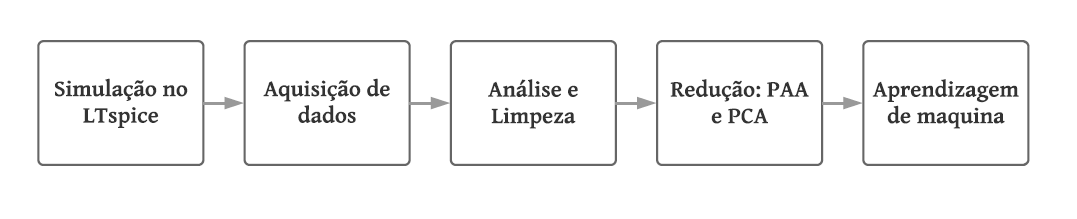
\includegraphics[width=13cm]{./02_Cap1/figures/diagrama.PNG}
\caption{\label{fig:diagrama}- Diagrama do fluxo de informação dos dados}
\end{center}
\end{figure}


